


\section{Solution}
\label{solution}

Our solution to improve throughput per unitary cost when doing model inference first starts by being able to dynamically choose between different types of hardware with a variance of unitary cost per hour, for this we show an initial simplified version that only selects between a CPU VM and one type of rented GPU, but this should easily be expanded to a bigger variety of hardware accelerators. When doing inference however, to easily switch between the accelerators without shutting down the microservice running the code, we choose to run the main application code separate from the model inference on the hardware accelerator, and thus we require a way to link the our interface to a possibly local execution in the case of CPU inference, or remote execution for GPU inference.


\subsection{Dynamic Module Selection}

To optimize throughput per unitary cost, we select different hardware accelerators based on current throughput and utilization characteristics.

\subsubsection{High Throughput and High Device Utilization (HDU)}

When the system operates at high throughput and thus high device utilization (HDU), GPUs should generally the optimal choice. GPUs should provide at high device utilization superior throughput per unitary cost and per watt (W) due to their parallel processing capabilities and the inherent parallelizability of deep learning model inference and training.
This makes them always suitable for training models, where high device utilization is a common scenario.

\subsubsection{Low Throughput and Low Device Utilization (LDU)}

In contrast, low throughput and low device utilization (LDU) may be encountered during inference, especially for rarely accessed models like those hosted on platforms such as Hugging Face. In these scenarios, CPUs emerge as the more cost-effective option. CPUs should offer better throughput per unitary cost in LDU conditions because they consume less power when idle or underutilized, and their energy requirements do not scale as drastically as GPUs.

Considering energy consumption from a holistic perspective\textemdash{}factoring in the energy used by the orchestrator or main CPU server in addition to the GPU\textemdash{}CPUs may also demonstrate higher throughput per watt. This is particularly true in architectures where separate servers are used for orchestration and computation. 

To implement this we obtain throughput per unitary cost profiles of each of the possible hardware types from a historical throughput profiles data source and select the lowest unitary cost for our current inference throughput, we outline the final architecture for this dynamic selection in section \ref{optimized-solution}.


 As we discussed in section \ref{solution}, our solution separates the inference hardware accelerators from the main microservice component to prevent it from being shutdown, thus we require a way to link these the main microservice component with the inference hardware accelerator components, to do this we propose an initial solution based on dynamic linking with WebAssembly primitives, and then improve on this initial proposal's performance bottlenecks by using modern WebAssembly component model infrastructure.

\subsection{Remote Module Execution with Dynamic Linking}
Our initial solution for remote module execution uses WASI v1 and Wasmtime runtime abstractions, such as \textbf{Store}, \textbf{Linker}, and \textbf{Module}, to implement dynamic linking. This involves manually handling shared libraries, memory, and tables.

Before implementing remote module execution, first we require a dynamic linking implementation for linking modules since WASI v1 does not implement this.

% Dynamic linking steps:

% 1 - Create Store and Linker 
% 2 - populate linker with (dlopen, dlsym, dlerror)
% 3 - if required table and memory is created and store references in linker
% 4- read dylink section of main module, extract shared library dependencies and for each shared library do step 4 through 7.
% 5 - Extract from current module dylink section memory size, memory alignment, table size, and table requirements alignment, expand memory and table accordingly.
% 5 - read share library dependencies, execute step 4 recursively.
% 6 - Instantiate current module with linker, which resolves all imports automatically.
% 7 - Obtain exports from the instantiated module and place their references in linker.
% 8 - Now get the main instantiated module and call it's entry function

\subsubsection{Application Compilation}
To create these modules, we use the WASI SDK compiler toolchain with -fPIC, -shared and -Wl,--export-all flags to compile our shared libraries.
%TODO: Why is position independent code required for the shared library? What happens if the flag is not set? Explain%
The -fPIC Flag makes sure the compiler generates position independent WASM code, the -shared flag generates the shared library and the -Wl,--export-all flag makes sure the linker exports all symbols even if unused. After compiling the shared libraries, we use also compile the main module as a shared library.

\subsubsection {Dynamic Linking Approaches}
There are multiple approaches to dynamic linking, such as shared-nothing dynamic linking, shared-something dynamic linking, and shared-everything dynamic linking.

\subsubsection{Shared-Nothing Dynamic Linking}

Shared-nothing dynamic linking architecture is an approach to dynamic linking that does not allow for the sharing of resources between modules other than with explicit communication. This approach is used in the Component Model, which is a part of the WebAssembly System Interface (WASI) v2 standard. The Component Model is an abstraction above WebAssembly modules that allows communication between components of two different languages. It adds common types for lists, strings, etc., which differ between languages to enable this communication. The Components Model forces the developer to specify an interface (thus the explicit communication) that only contain immutable copied values, opaque typed handles and immutable uninstantiated modules, and also fully encapsulates linear memories, tables and globals, thus it does not allow for shared resources between modules.

The main advantage of shared-nothing dynamic linking is that it provides strong isolation between modules, modules cannot accidently or maliciously access each other's resources. However, this isolation comes at the cost of performance, as it requires explicit communication between modules to share resources and can lead to increased memory usage due to the duplication of resources.

\subsubsection{Shared-Everything Dynamic Linking}

Shared-everything dynamic linking architecture is an approach to dynamic linking that allows for the sharing of all resources between modules. This includes the function table, memory, and global variables. This approach is used in the WebAssembly dynamic linking proposal, which is a part of the WebAssembly System Interface (WASI) standard. The proposal defines a new section in the WebAssembly binary format called `dylink.0` that contains the information required to determine the shared library's dependencies, memory and function table requirements, and load them at runtime with the standard `dlopen`/`dlsym` functions.


\subsubsection{Dynamic Linking Implementation}

We base our dynamic linking implementation on existing work \cite{makitalo2021bringing} that was done for the EMScripten compiler toolchain and not the WASI SDK compiler toolchain. This work focused on runtime dynamic linking with dlopen, dlsym, dlerror symbols, while ours will be focused on load time dynamic linking.

As a base we use the WASMTime runtime API in Rust, which gives use abstractions for WebAssembly objects such as Table, Memory, Module, Instance, and also other relevant abstractions such as a Linker for linking imports and exports of multiple module or Store, which stores references to instances, functions, etc..

To implement load time dynamic linking, we start by creating the Store and Linker objects. After that we create Table and Memory objects and store their references in the linker. To know what shared library dependencies the main module requires, we read the dylink.0 section of the WASM Binary and extract them from the WASM\_DYLINK\_NEEDED subsection as specified in the \href{https://github.com/WebAssembly/tool-conventions/blob/main/DynamicLinking.md}{Dynamic Linking Spec}. Now for each module recursively, we extract from the dylink.0 section the memory size requirements, memory alignment, table size, table alignment and expand the Memory and Table accordingly. We then instantiate each module with the linker, which resolves all the imports automatically. We then obtain the exports of the instantiated module and place their references in the linker. This procedure must be done recursively such that we only instantiate a module with dependencies after its dependencies have already been instantiated.

\subsubsection{Remote Module Execution}

To enable remote execution of these shared libraries however, due to these shared libraries not enforcing an immutable layer, the memory must be shared.

This solution for remote module execution, as can be seen in figure \ref{fig:dynamic-linking-arch}, thus brings significant performance bottlenecks due to shared memory between the servers.

\begin{figure}[h!]
\centering
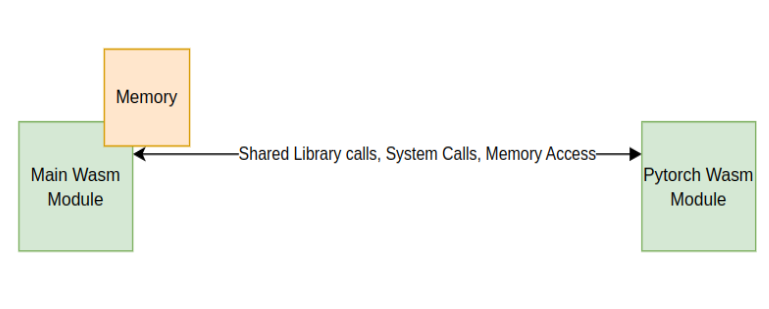
\includegraphics[width=1.0\textwidth]{Images/dynamic-linking-arch.png}
\caption{Architecture for remote module execution with shared memory.}
\label{fig:dynamic-linking-arch}
\end{figure}


\subsection{Remote Module Execution with Component Model and wRPC}
\label{optimized-solution}
The second solution represented in Figure \ref{fig:architecture}, builds on the Component Model and wRPC, by enforcing \textbf{shared-nothing} principles and leveraging the immutable high-level WIT interfaces from the component model, this approach eliminates the need of sharing memory between the components.

\begin{itemize}
\item Components communicate explicitly via immutable WIT interfaces, and each component has it's own linear memory.
\item Remote execution is enabled through wRPC
\end{itemize}

\begin{figure}[h!]
\centering
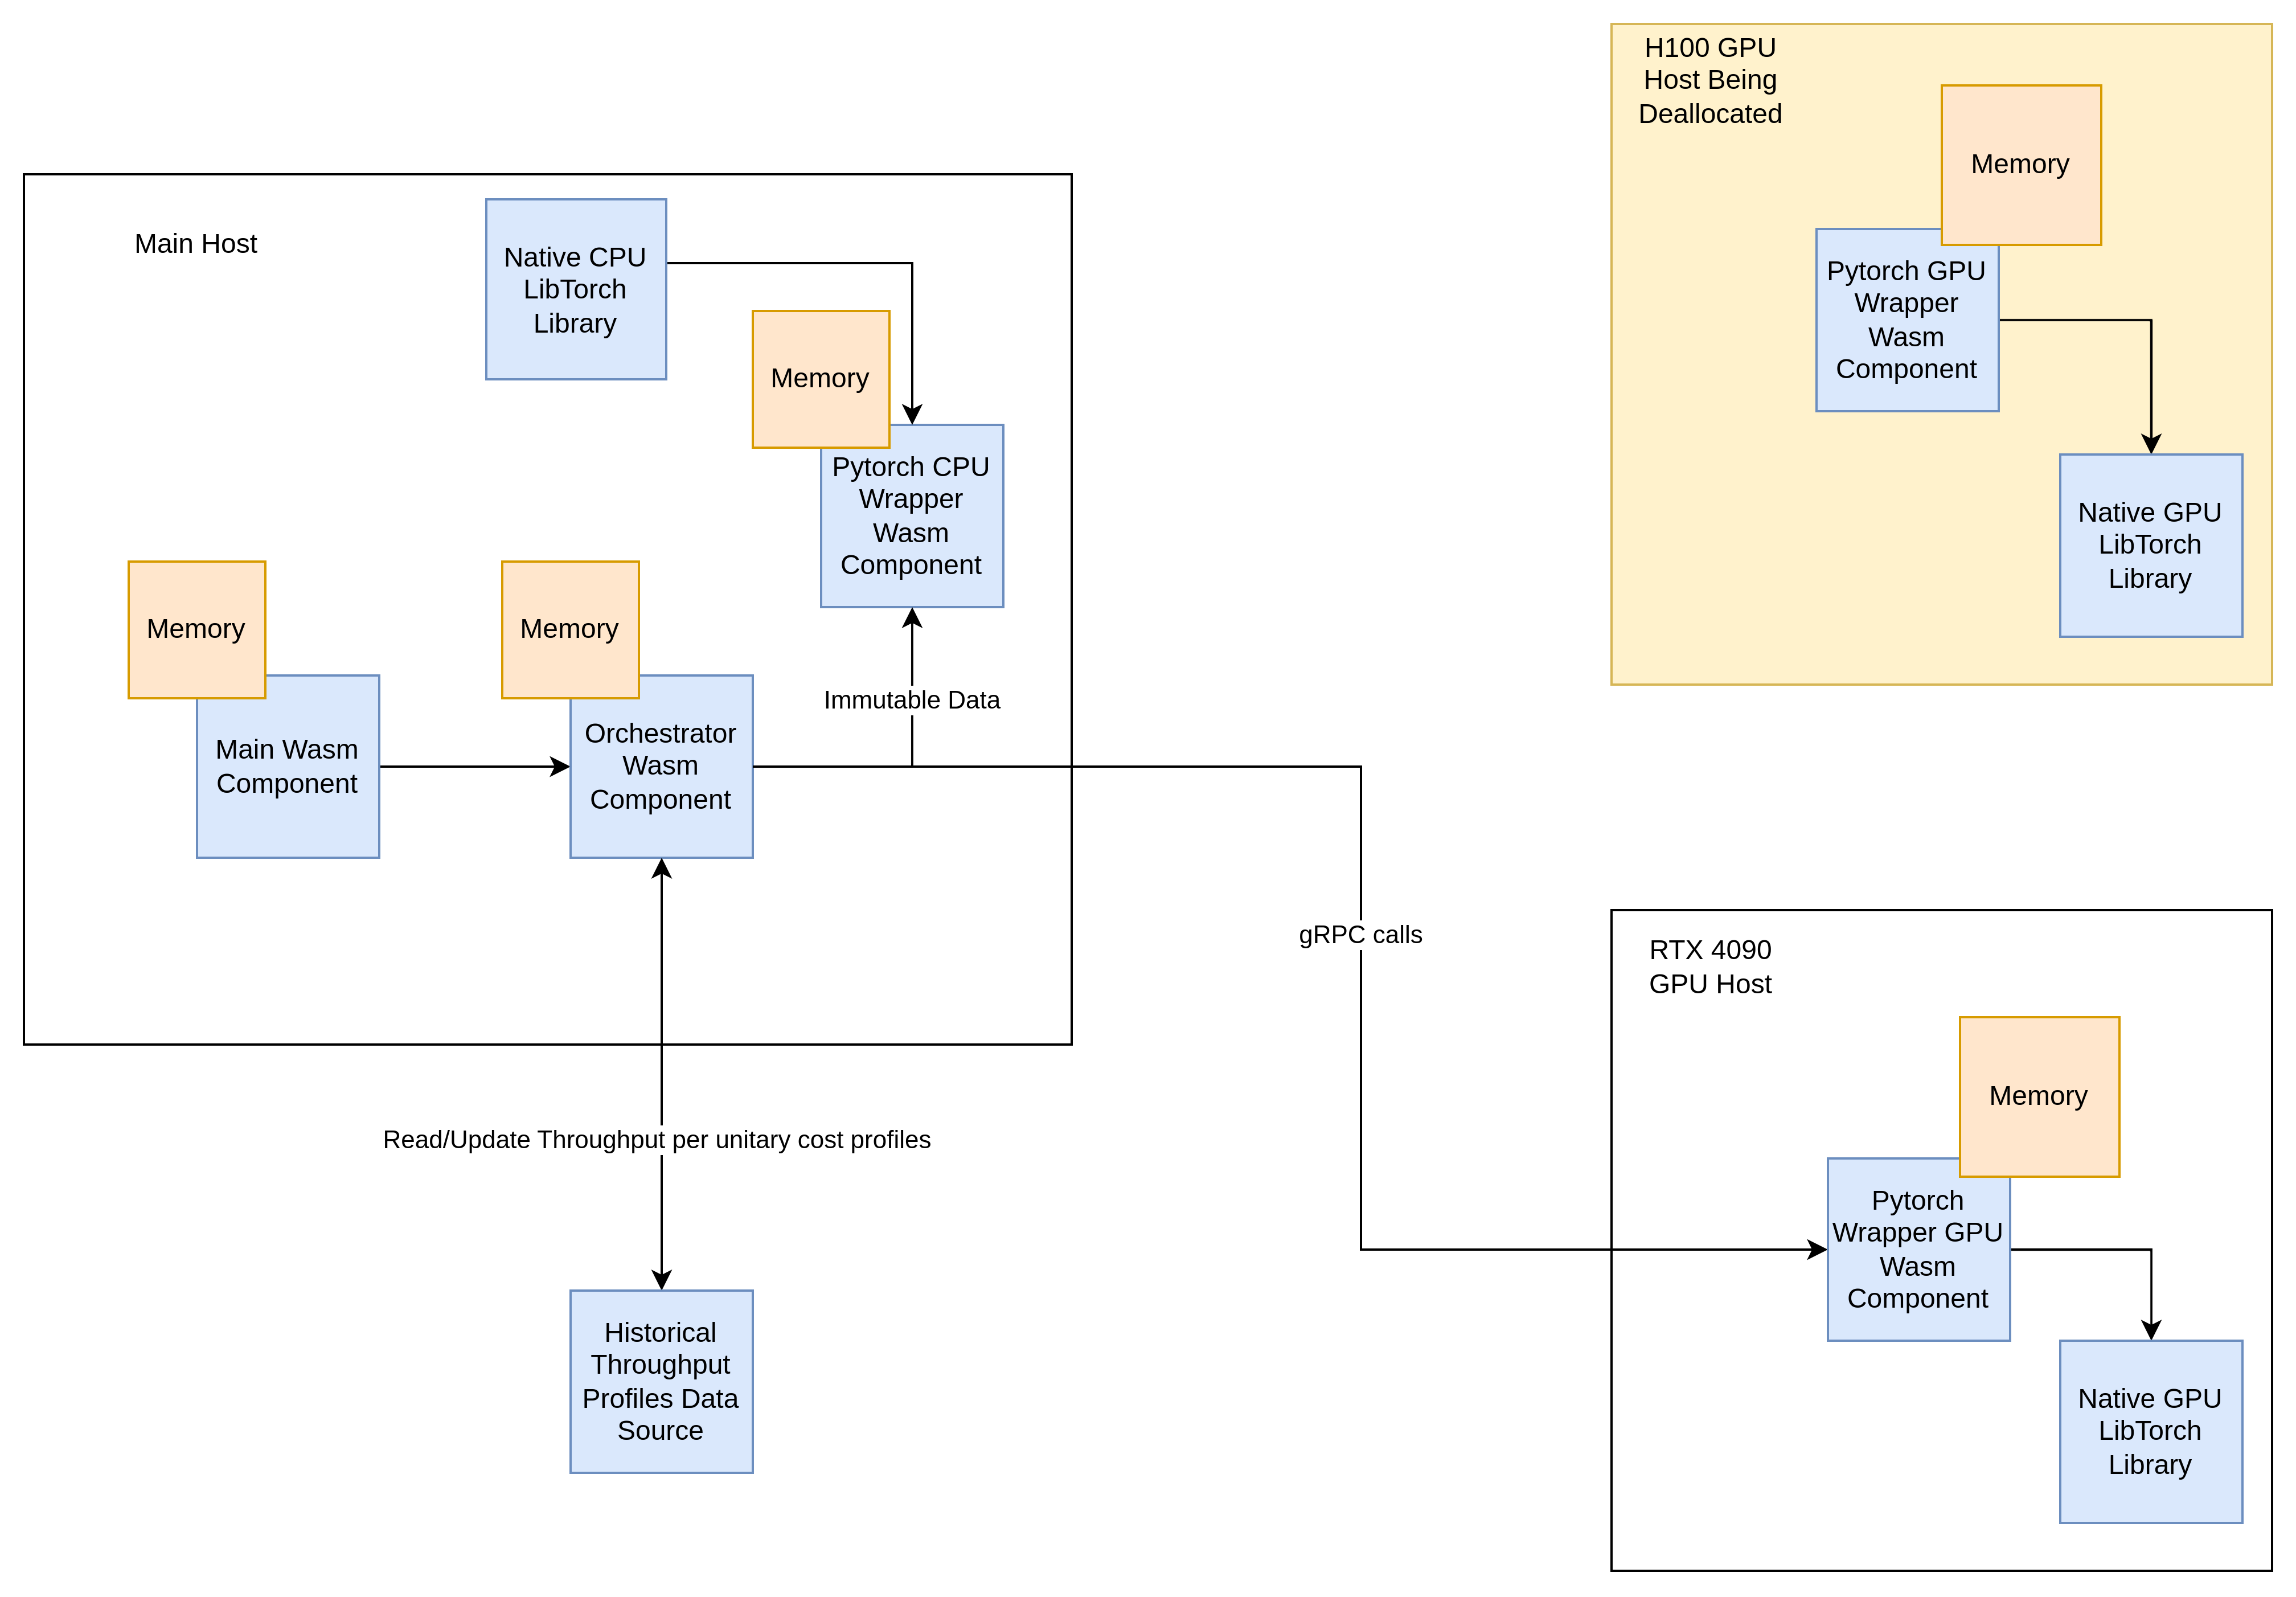
\includegraphics[width=1.0\textwidth]{Images/component-model-arch.png}
\caption{System architecture for dynamic selection of accelerators based on workload. }
\label{fig:architecture}
\end{figure}


\textbf{Steps for implementation}:
\begin{enumerate}
\item Compile shared libraries and main modules as WebAssembly components.
\item Use wRPC to establish communication between components.
\item Dynamically load components at runtime and resolve their interfaces.
\item Enable remote function execution using wRPC across distributed environments.
\end{enumerate}



By dynamically selecting the appropriate accelerator based on throughput and device utilization, we believe lower costs and possible energy savings can be achieved. 
The use of the standardized WASI v2 infrastructure, which allows interoperability between languages due to the WIT interface, flexibility in distributing the components across servers with the wRPC protocol, and not having the performance bottlenecks of the first solution derived from the shared memory, this provides the necessary abstraction to enable this dynamic selection seamlessly.


\pagebreak
% \section{Conclusion}
% We presented two solutions for dynamic linking in WebAssembly. The first, using WASI v1, offers a manual but functional implementation. The second, leveraging the Component Model and wRPC, provides a streamlined and efficient solution that balances performance, isolation, and scalability. These approaches enable dynamic linking and remote execution, paving the way for advanced, flexible, and distributed WebAssembly applications.